\subsection{Analyse der roten $\sigma$-Linien}
Die Aufspaltung der roten Spektrallinie ist in \autoref{fig: aufspaltung_rot} dargestellt. Zur quantitativen Analyse der Auspaltung wird das
Resultat unter anliegendem Strom von $I = \SI{10}{\ampere}$ verwendet. Gemäß Formel~\eqref{eq: fitfuntion_hysterese} bedingt dieser
eine magnetische Flussdichte von $B = \SI{587(3)}{\milli\tesla}$.

Die Helligkeit in Abhängigkeit von der horizontalen Position auf den aufgenommenen Bilder ist in \autoref{fig: rot_intensität} für das unaufgespaltene
und aufgespaltene Beugungsbild dargestellt. Anhand dessen werden die Positionen von $12$ Intensitätsmaxima und ihrer Aufspaltungen
vermessen. Die Daten sind in \autoref{tab: peaks_rot} aufgeführt. Eine graphische Darstellung der abgelesenen Intensitätsmaxima befindet sich in
den Abbildungen~\ref{fig: peaks_rot_0} und~\ref{fig: peaks_rot_10}.

Die für die Berechnung der Wellenlängenänderung relevanten Abstände $\symup{\Delta} s_i$ und $\symup{\Delta} s_i$ sind in \autoref{tab: abstände_rot}
aufgeführt. Mit Hilfe der Gleichungen~\label{eq: wellen_änderung}, \label{eq:energie_diff} und \label{eq: uebergangs_lande}
berechnen sich hieraus die Wellenlängenaufspaltung $\symup{\Delta} \lambda$, die
Energieaufspaltung $\symup{\Delta} E$ und schließlich die Werte für die Übergangs-Landé-Faktoren $g$. Alle Ergebnisse sind ebenfalls in
\autoref{tab: abstände_rot} eingetragen. Als Mittelwert für den Landé-Faktor ergibt sich
\begin{equation}
  g_{ij} = \num{1.045(5)}.
\end{equation}
\begin{figure}
  \centering
  \includegraphics[width = 0.7\textwidth]{../Messdaten/bilder_v27/messung_1_rot_sigma/aufspaltung_rot.png}
  \caption{Aufgenommene Intensitätsstreifen des roten Lichtes unter (von oben nach unten) $\SI{0}{\ampere}$, $\SI{7.5}{\ampere}$ und $\SI{10}{\ampere}$.}
  \label{fig: aufspaltung_rot}
\end{figure}
\begin{figure}
  \centering
  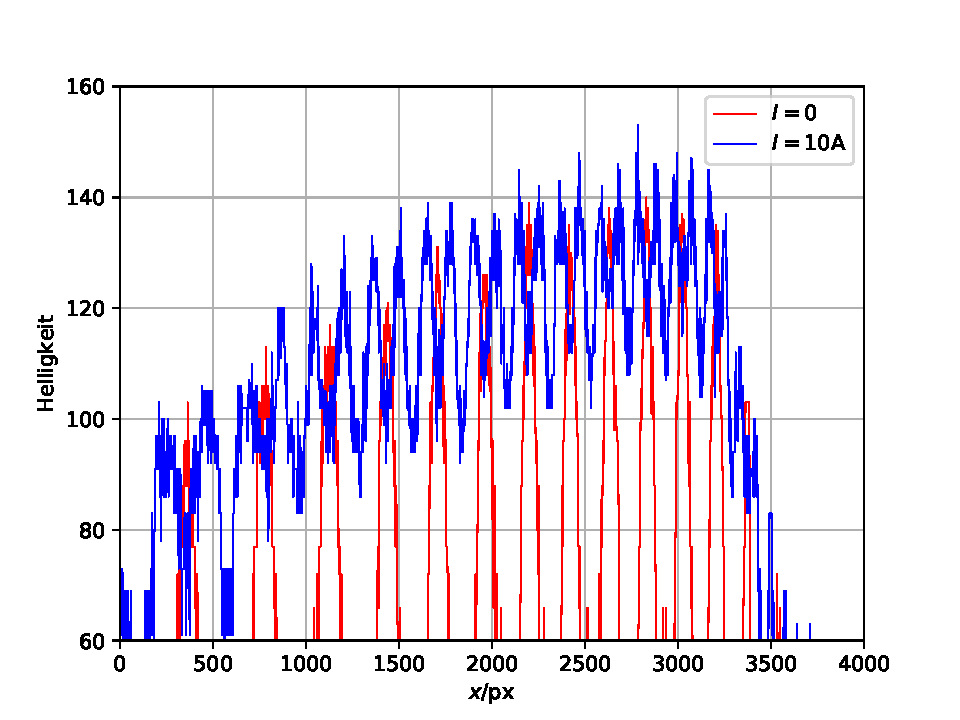
\includegraphics[width = 0.7\textwidth]{../Messdaten/plots/rot_sigma_intensitaet.pdf}
  \caption{Darstellung der Helligkeit der roten Linien in Abhängigkeit von der horizontalen Lage auf dem Foto.}
  \label{fig: rot_intensität}
\end{figure}
\begin{table}
\centering
\caption{Positionen $x_0$ und $x_{10}$ der Intensitätsmaxima unter $I= \SI{0}{\ampere}$ und $I= \SI{10}{\ampere}$.}
\label{tab: peaks_rot}
\begin{tabular}{S S[table-format=4.0] S[table-format=4.0] }
\toprule
{$x_0 /$ px} & \multicolumn{2}{c}{$x_{10} \:/\: $px} \\
\midrule
364 & 234 & 2145\\
784 & 470 & 2254\\
1132 & 693 & 2376\\
1436 & 865 & 2471\\
1705 & 1029 & 2579\\
1964 & 1207 & 2676\\
2201 & 1360 & 2782\\
2415 & 1511 & 2877\\
2632 & 1653 & 2980\\
2830 & 1775 & 3069\\
3022 & 1900 & 3166\\
3205 & 2017 & 3255\\
\bottomrule
\end{tabular}
\end{table}

\begin{figure}
  \centering
  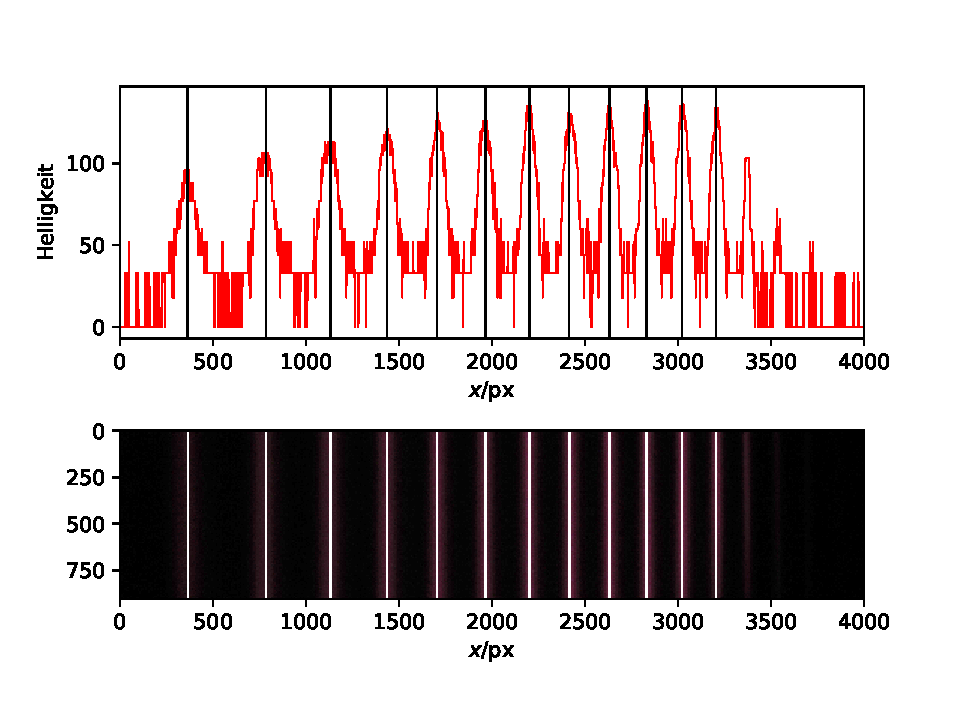
\includegraphics[width = 0.7\textwidth]{../Messdaten/plots/peaks_rot_sigma_0.pdf}
  \caption{Darstellung der abgelesenen Lagen der Intesitätsmaxima für das Beugungsbild unter $I =\SI{0}{\ampere}$.}
  \label{fig: peaks_rot_0}
\end{figure}
\begin{figure}
  \centering
  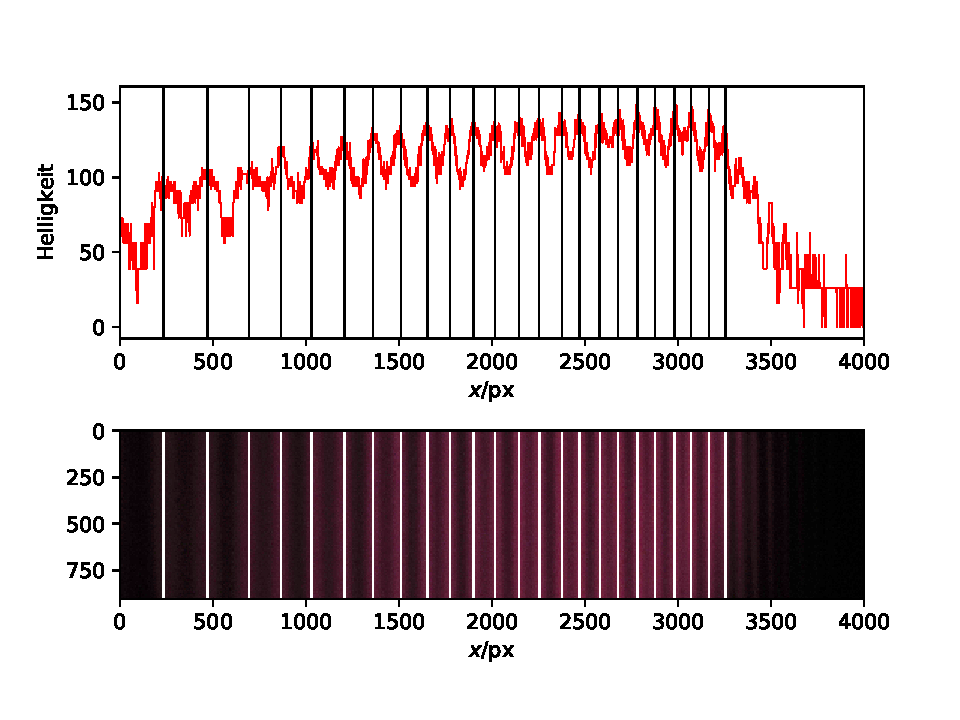
\includegraphics[width = 0.7\textwidth]{../Messdaten/plots/peaks_rot_sigma_10.pdf}
  \caption{Darstellung der abgelesenen Lagen der Intesitätsmaxima für das Beugungsbild unter $I =\SI{10}{\ampere}$.}
  \label{fig: peaks_rot_10}
\end{figure}
\input{../Messdaten/tabs/abstände_rot.tex}
